\begin{problem}
Критерий непрерывности в терминах односторонних пределов (Предложение 1, Лекция
13). Доказательство локальных свойств непрерывных функций. Доказательство теоремы
о композиции непрерывных функций.
\end{problem}
Предложение 1. $f \in C(a) \Leftrightarrow f$ непрерывна в а справа и слева, причём
$$
\lim _{x \rightarrow a+} f(x)=\lim _{x \rightarrow a-} f(x)=f(a) .
$$

Доказательство. Необходимость. Если $f \in C(a)$, то по первому определению непрерывности для любого $\varepsilon>0$ найдётся такое $\delta>0$, что при всех таких $x \in E$, что $|x-a|<\delta$ $|f(x)-f(a)|<\varepsilon$. Тогда при всех таких $x \in E$, что $-\delta<x-a<0$ выполнено $|f(x)-f(a)|<\varepsilon$, то есть функция $f$ непрерывна в точке $a$ слева. Непрерывность справа доказывается точно так же.

Достаточность. Непрерывность справа и слева означает, что для любого $\varepsilon>0$ найдётся такое $\delta_1>0$, что при всех таких $x \in E$, что $0<x-a<\delta_1|f(x)-f(a)|<\varepsilon$, а также найдётся такое $\delta_2>0$, что при всех таких $x \in E$, что $-\delta_2<x-a<0|f(x)-f(a)|<\varepsilon$. Тогда для $\delta=\min \left\{\delta_1, \delta_2\right\}$ при всех таких $x \in E$, что $|x-a|<\delta$ будет выполнено неравенство $|f(x)-f(a)|<\varepsilon$, то есть для любого $\varepsilon>0$ найдётся своё $\delta$, для которого выполнено определение непрерывности.
Предложение 2. (Локалъные свойства непрерывных функций). Пусть функции $f$ u $g$ определены на множестве $E, a \in E, f \in C(a), g \in C(a)$. Тогда выполнены следующие свойства:
1) $\alpha f+\beta g \in C(a) \forall \alpha, \beta \in \mathbb{R}$ (линейная комбинация непрерывных в точке функций является непрерывной в этой точке функцией;
2) $f \cdot g \in C(a)$ (произведение непрерывных в точке функций является функцией, непрерывной в этой точке);
3) если $g(x) \neq 0 \forall x \in E$, то $\frac{f}{g} \in C(a)$ (частное непрерывных в точке функций является функиией, непрерывной в этой точке);
4) $\exists M \geq 0, \delta>0: \forall x \in E \cap U_\delta(a)|f(x)| \leq M$ (для непрерывной в точке функции найдётся окрестность этой точки, в которой функиия ограничена);
5) если $f(a) \neq 0$, то существует такая окрестность $U_\delta(a)$ точки $а$, что
$$
|f(x)|>\frac{|f(a)|}{2} \forall x \in E \cap U_\delta(a),
$$

причём для таких $x f(x) \cdot f(a)>0$, то есть функция $f$ совпадает по знаку с $f(a)$.

Доказательство. В случае изолированной точки $а$ эти свойства следуют из того, что любая функция непрерывна в точке $a$. Если $a$ является предельной точкой, то свойства следуют из определения непрерывной функции через предел и арифметики пределов.
Предложение 3. (Теорема о композиции непрерывных функций). Пусть множества $E, D$ и $K$ содержатся в $\mathbb{R}, f: E \rightarrow D, g: D \rightarrow K$. Пусть $a \in E, f(a) \in D$, $u f \in C(a), g \in C(f(a))$. Тогда функция $g \circ f: E \rightarrow K$ непрерывна в точке а (здесь $(g \circ f)(x):=g(f(x)))$.

Доказательство. Пусть $a_n \in E \forall n \in \mathbb{N}, a_n \rightarrow a$. Тогда $f\left(a_n\right) \in D$ и в силу непрерывности (см. определение непрерывности по Гейне) $f\left(a_n\right) \rightarrow f(a), n \rightarrow a$. Так как $g$ непрерывна в точке $f(a)$, то опять же по определению непрерывности по Гейне имеем
$$
\lim _{n \rightarrow \infty} g\left(f\left(a_n\right)\right)=g(f(a)) .
$$

\newpage
\begin{problem}
Примеры устранимых разрывов и разрывов 1 и 2 рода. Пример функции, разрывной в
каждой точке. Разрывы функции, монотонной на интервале (Предложения 4, Лекция 13).
\end{problem}
Примером функции с точкой устранимого разрыва может служить $f(x)=\frac{\sin x}{x}$, если $x \neq 0$ и $f(0)=0$, где $a=0$. Эта функция в точке $a=0$ имеет значение 0 , а предел при $x \rightarrow 0$ равен 1 , поэтому достаточно положить $f(0)=1$, чтобы функция $f$ стала непрерывной в точке 0 .

Во-вторых, в точке $a \in E$ у функции может не быть предела, но при этом существуют оба односторонних предела (см. предыдущую лекцию), которые не равны друг другу. В этом случае точка $a$ называется точкой разрыва первого рода. Иногда такой разрыв называют скачком. Примером функции с такой точкой разрыва может служить кусочно заданная функция $f(x)=\left\{\begin{array}{l}-1, \text { если } x<0, \\ 1, \text { если } x \geq 0 .\end{array}\right.$ Точка $a=0$ является точкой разрыва первого рода. См. также рис. 2.

В-третьих, хотя бы один из односторонних пределов в точке $f \in E$ может не существовать или быть равным $\pm \infty$ (то есть либо $+\infty$, либо $-\infty$, либо просто $\infty$.) Такая точка называется точкой разрыва второго рода. Точку разрыва этого типа имеет в нуле гипербола $f(x)=\frac{1}{x}$ (если доопределить её в нуле любым действительным числом), так как $\lim _{x \rightarrow 0-0} \frac{1}{x}=-\infty$

Дирихле $D(x)$ (см. прошлые лекции) не имеет предела ни в одной точке, поэтому она является примером функции, разрывной в каждой точке. Все точки области определения функции Дирихле являются точками разрыва второго рода.

Предложение 4. Монотонная на интервале функция может иметь на этом интервале только разрывы первого рода.

Доказательство. Пусть функция $f$ не убывает на интервале $(a, b)$ (случай невозрастания сводится к случаю неубывания заменой функции $f$ на $-f$.) Число $f\left(x_0\right)$ является верхней гранью для множества значений $f$ в точках $x \in\left(a, x_0\right)$ и нижней гранью для множества значений $f$ в точках $x \in x_0$. Поэтому для любой точки $x_0 \in(a, b)$ имеем в силу теоремы Вейерштрасса:
$$
\lim _{x \rightarrow x_0-0} f(x)=\sup _{x<x_0} f(x) \leq f\left(x_0\right) \leq \inf _{x>x_0} f(x)=\lim _{x \rightarrow x_0+0} f(x) .
$$

Таким образом, в любой точке интервала $(a, b)$ существуют односторонние пределы, но они могут не совпадать, что возможно лишь при разрывах первого рода.

\newpage
\begin{problem}
Доказательство теоремы о нуле непрерывной на отрезке функции (Теорема 1, Лекция
13). Доказательство 1-й теоремы Вейерштрасса.
\end{problem}
Теорема 1. Пусть функция $f \in C([a, b])$ u $f(a) \cdot f(b)<0$. Тогда $\exists c \in[a, b]: f(c)=0$.
Доказательство. По условию функция $f$ принимает значения разных знаков в точках $a$ и $b$. Пусть, например, $f(a)<0$, тогда $f(b)>0$. Разобъём отрезок $[a, b]$ пополам. Если $f\left(\frac{a+b}{2}\right)=0$, то всё доказано, а если нет, то пусть,например, $f\left(\frac{a+b}{2}\right)<0$. Обозначим $\frac{a+b}{2}$ через $a_1$, а $b$ через $b_1$. Для отрезка $\left[a_1, b_1\right]$ проделаем ту же самую процедуру: возьмём точку $\frac{a_1+b_1}{2}$, найдём $f\left(\frac{a_1+b_1}{2}\right)$; если это значение не равно нулю, то из отрезков $\left[a_1, \frac{a_1+b_1}{2}\right]$ и $\left[\frac{a_1+b_1}{2}, b_1\right]$ выберем тот, на концах которого функция $f$ принимает значения разных знаков. Обозначим через $a_2$ левый конец этого отрезка, а через $b_2$ - правый. Разобъём этот отрезок пополам и т.д.. Если ни в какой из середин отрезков не получится нулевое значение функции, тот этот процесс будем продолжать до бесконечности и получим последовательность стягивающихся отрезков. Пересечение этих отрезков состоит, как мы знаем, из одной точки, которую обозначим через $c$. Последовательность левых концов построенных отрезков $\left\{a_n\right\}_{n=1}^{+\infty}$ и последовательность правых концов $\left\{b_n\right\}_{n=1}^{+\infty}$ стремятся к $c$, поэтому, в силу непрерывности функции на отрезке $[a, b] f\left(a_n\right) \rightarrow f(c), f\left(b_n\right) \rightarrow f(c)$ и при этом $f\left(a_n\right) \cdot f\left(b_n\right)<0$ по построению. Используя предельный переход в неравенствах и арифметику предела, имеем: $f^2(c)=\lim _{n \rightarrow \infty} f\left(a_n\right) \cdot f\left(b_n\right) \leq 0$, поэтому $f(c)=0$, чем все и доказано.

Теорема 2. (1-я теорема Вейеритрасса.) Пусть функиия $f$ определена и непрерывна на отрезке $[a, b]$. Тогда она ограничена на этом отрезке.

Доказательство. Если функция $f$ не ограничена на отрезке, то для каждого натурального $n$ существует такая точка $x_n \in[a, b]$, что $\left|f\left(x_n\right)\right|>n$. Все элементы последовательности $\left\{x_n\right\}_{n=1}^{+\infty}$ принадлежат отрезку $[a, b]$, то есть последовательность ограничена, поэтому по теореме Больцано - Вейерштрасса она имеет хотя бы одну сходящуюся к некоторому числу $c$ подпоследовательность $c_k=a_{n_k}$, причём $c \in[a, b]$ в силу предельного перехода в неравенствах. При этом $\left|f\left(c_k\right)\right|>n_k$, поэтому в точке $c$ у функции $f$ не существует конечного предела, что противоречит непрерывности этой функции.

Отметим, что можно было доказать эту теорему и с помощью принципа Бореля - Лебега, используя локальную ограниченность непрерывной функции. Действительно, для каждой точки отрезка $[a, b]$ существует окрестность, в которой функция $f$ ограничена. Такие окрестности образуют покрытие отрезка $[a, b]$, а тогда по принципу Бореля - Лебега мы можем выбрать конечное подпокрытие, на каждом элементе которого функция $f$ ограничена. Тогда мы можем из всех чисел, которыми ограничена функция, выбрать максимальное, а этим числом функция будет ограничена уже на всём отрезке.

\newpage
\begin{problem}
Доказательство 2-й теоремы Вейерштрасса. Примеры, демонстрирующие важность условий про непрерывность и отрезок в теоремах Вейерштрасса. Доказательство теоремы
Больцано – Коши о промежуточном значении.
\end{problem}
Теорема 3. (2 теорема Вейерштрасса.) Пусть функция $f$ определена и непрерывна
на отрезке $[a, b]$. Тогда существуют такие точки $x_1, x_2 \in[a, b]$, что
$$
f\left(x_1\right)=m=\inf _{a \leq x \leq b} f(x), f\left(x_2\right)=M=\sup _{a \leq x \leq b} f(x) .
$$

Доказательство. Существование точных верхней и нижней граней функции $f$ следует из того, что по первой теореме Вейерштрасса $f$ ограничена на отрезке $[a, b]$, то есть множество её значений ограничено, а тогда существует точная верхняя и точная нижняя грани её множества значений.

Доказательство проведём для супремума. Предположим, что точка $x_2$ не найдётся. Тогда $M-f(x)>0 \forall x \in[a, b]$. Рассмотрим функцию $g$, которая в точке $x \in[a, b]$ принимает значение $\frac{1}{M-f(x)}$. В силу локальных свойств непрерывных функций $g$ непрерывна в каждой точке отрезка $[a, b]$, а тогда она непрерывна на всём отрезке по определению, что даёт её ограниченность на всём отрезке по 1-й теореме Вейерштрасса. С другой стороны, по определению супремума
$$
\forall \varepsilon>0 \exists x_{\varepsilon} \in[a, b]: \quad f\left(x_{\varepsilon}\right)>M-\varepsilon .
$$

При $\varepsilon=1 / n$ получим, что $\forall n \in \mathbb{N} g\left(x_{1 / n}\right)>n$, то есть функция $g$ не ограничена на отрезке. Таким образом, пришли к противоречию.

Пример 2. 1) Пусть $f(x)=\frac{1}{x}, x \in(0,1)$. Тогдa $\inf _{0<x<1} f(x)=1, a \sup _{0<x<1} f(x)=+\infty$. Мы видим, что функция $f$ непрерьвна на интервале, но не являтея ограниченной и не достигает точной верхней и точной нижней грани. Причина этого - то, что функция определена на интервале, а не отрезке.
2) Пусть $f(x)=\left\{\begin{array}{l}x, 0<x \leq 1, \\ \frac{1}{2}, x=0 .\end{array}\right.$ Тогда $\inf _{0 \leq x \leq 1} f(x)=0, a \sup _{0 \leq x \leq 1} f(x)=1=f(1)$. Здесъ нет точки, в которой значение функции равно точной нижней грани, так как функция не является непрерывой на отрезке, хотя и определена на отрезке. График этой функции изображён ниже.
Теорема 4. (Коши о непрерывной функции.) Пусть функция $f$ определена и непрерывна на отрезке $[a, b], m=\inf _{a \leq x \leq b} f(x), M=\sup _{a \leq x \leq b} f(x)$. Тогда для любого числа $C \in[m, M]$ существует такая точка $c \in[a, b]$, что $f(c)=C$.

Доказательство. Если $C=m$ или $C=M$, то всё доказано в теореме 3. Будем использовать обозначения этой теоремы. Если $C \in(m, M)$, то функция $g:=f-C$ непрерывна на отрезке $\left[x_1, x_2\right]$ (отрезок неориентированный) и $g\left(x_1\right)=m-C<0$, а $g\left(x_2\right)=M-C>0$, то есть для функции $g$ на отрезке $\left[x_1, x_2\right]$ выполнены все условия теоремы 1 . Тогда
$$
\exists c \in\left[x_1, x_2\right]: g(c)=0,
$$

то есть $f(c)=C$.
\newpage

\begin{problem}
Примеры равномерно непрерывных и неравномерно непрерывных функций (Лекция
14). Доказательство теоремы Гейне – Кантора (любое).
\end{problem}

\begin{example}
    1) Функция $f(x)=\sin x, x \in \R$
    равномерно непрерывна на $\R,$ т. к.
    $\forall \varepsilon>0$
    имеем: $|\sin x-\sin y|=
        |2\sin\frac{x-y}{2}\cos\frac{x+y}{2}|
        \leq2|\sin\frac{x-y}{2}|\leq|x-y|<\varepsilon,$
    если $|x-y|<\delta,$ где $\delta=
        \varepsilon.$ Таким образом, здесь выбор
    $\delta$ не зависит от точек на вещественной
    оси, а зависит только от $\varepsilon.$\\
    2) Функция $f(x)=\sin\frac{1}{x}, x > 0$
    не является равномерно непрерывной на $\R_+,$
    так как точки вида $x=\frac{1}{\frac{\pi}{2}+
            2\pi n}$ и $y=\frac{1}{-\frac{\pi}{2}+2\pi n}$
    ($n \in \N$) могут быть сколь угодно близки
    друг к другу при достаточно больших $n,$
    но $|\sin\frac{1}{x}-\sin\frac{1}{y}|=2$
    при всех натуральных $n,$ то есть при
    $0<\varepsilon<2$ необходимо будет подбирать
    $\delta$ в зависимости от конкретной точки.
    Рисунок 3 ниже демонстрирует это.
    Красная часть графика пересекает верхнюю
    и нижнюю стороны одного из
    прямоугольников. Чтобы этого не было,
    нужно уменьшить длину $\delta$ горизонтальной
    стороны при приближении к нулю. Это значит,
    что равномерной непрерывности нет.\begin{figure}[h!]
        \center{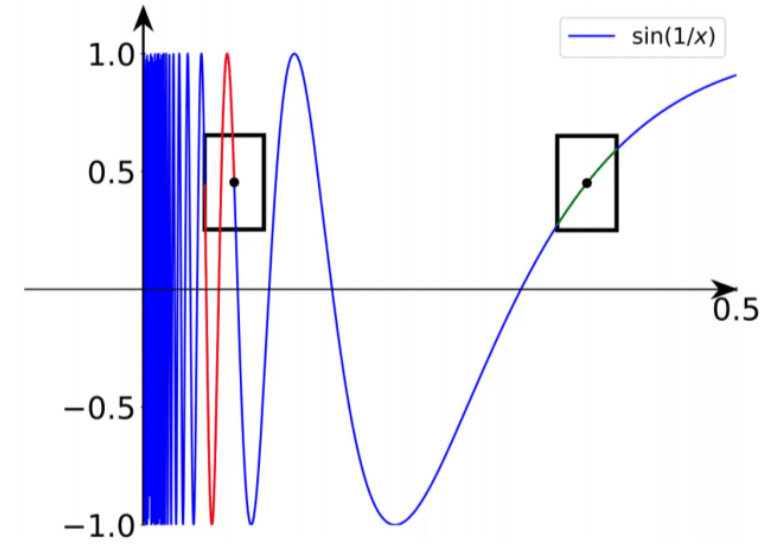
\includegraphics[scale=0.5]{sin1x.png}}
        \caption{Чем ближе к нулю, тем быстрее растёт функция на промежутках монотонности.}
        \label{fig:image}
    \end{figure}
\end{example}

\begin{theorem}(\textbf{Гейне -- Кантора о равномерной
        непрерывности}).
    Функция $f,$ непрерывная на отрезке $[a, b],$
    равномерно непрерывна на этом отрезке.
\end{theorem}
\begin{proof} \textbf{(1-й способ, через
        принцип Бореля -- Лебега).}
    По условию функция $f$ непрерывна в каждой точке
    отрезка $[a, b],$ поэтому в силу критерия Коши
    для функций при всяком $\varepsilon>0$
    для каждой точки $x\in[a, b]$
    найдётся такая окрестность $U_{\delta}(x),$
    что при всех $x, y\in\;U_{\delta}(x)$
    выполнено неравенство $|f(x)-f(y)|<\varepsilon.$
    Отметим, что $\delta$ зависит от точки
    $x,$ то есть для разных точек найдутся,
    вообще говоря, разные $\delta.$
    Все окрестности вида $U_{\delta/2}(x)$покрывают
    отрезок $[a, b],$ так как каждая
    точка отрезка принадлежит
    какой-нибудь из этих окрестностей.

    По принципу Бореля -- Лебега из
    системы всех окрестностей можно
    выбрать конечную систему,
    также покрывающую отрезок $[a, b].$
    Обозначим эти окрестности
    $$
        U_{\delta_i/2}(x_i),
        \textrm{ где } i=1,\;2,\;...,\;n.
    $$
    Положим
    $\delta=\min\{\frac{\delta_1}{2},\;
        \frac{\delta_2}{2},\;...,\;\frac{\delta_n}{2}\}$
    и докажем, что для любых таких точек $x',\;
        x''\in\;[a, b],$ что $|x'-x''|<\delta,$
    справедливо неравенство $|f(x')-f(x'')|
        <\varepsilon.$ Действительно, так как
    окрестности $\{U_{\delta_i/2}
        (x_i)\}_{i=1}^n$ покрывают
    отрезок $[a, b],$ то найдётся
    такая окрестность
    $$
        U_{\delta_j/2(x_j)},\;
        \textrm{ что }
        x'\in U_{\delta_j/2}.
    $$
    Тогда
    $$
        |x''-x_j|\leq|x'-x_j|+|x''-x'|<\delta_j/2+
        \delta\leq\delta_j,
    $$
    то есть $x''\in\;U_{\delta_j}(x_j),$
    поэтому, вспоминая, как были построены
    все окрестности вида $U_{\delta}(x),$
    мы имеем $|f(x')-f(x'')|<\varepsilon.$
    Таким образом, равномерная непрерывность
    доказана.
\end{proof}
\begin{proof} \textbf{(2-й способ, через
        теорему Больцано -- Вейерштрасса).}
    Предположим, что функция $f$ не является равномерно
    непрерывной на отрезке $[a, b].$
    Тогда существует такое $\varepsilon_1>0,$ что для любого
    натурального $n$ найдутся такие точки
    $x_n\in[a, b]$ и $y_n\in[a, b],$ что $|x_n-y_n|
        <\frac{1}{n},$ но
    $$
        |f(x_n)-f(y_n)|\geq\varepsilon_1. \eqno(1)
    $$
    Все элементы последовательностей $\{x_n\}_{n=1}^{\infty}$
    и $\{y_n\}_{n=1}^{\infty}$ принадлежат
    отрезку $[a, b],$ поэтому в силу теоремы Больцано --
    Вейерштрасса из них можно выбрать
    сходящиеся подпоследовательности
    $\{x_{n_k}\}_{k=1}^{\infty}$ и
    $\{y_{n_k}\}_{k=1}^{\infty}.$
    Так как при $n\rightarrow\infty$
    $|x_n-y_n|\rightarrow0,$ то пределы
    этих подпоследовательностей при $k\rightarrow
        \infty$ совпадают. Пусть эти пределы
    равны $x_0.$ $x_0\in[a, b]$ по предельному
    переходу в неравенствах, а тогда по условию
    функция $f$ непрерывна в точке $x_0.$
    В силу определения по Гейне непрерывной функции
    при любом $\varepsilon>0$ $|f(x_{n_k})-f(x_0)|
        <\frac{\varepsilon}{2}$ и $|f(y_{n_k})-f(x_0)|
        <\frac{\varepsilon}{2}.$ Если взять
    $\varepsilon=\varepsilon_1,$ то
    получим цепочку неравенств:
    $$
        \varepsilon_1 > |f(x_{n_k})-f(x_0)|+
        |f(y_{n_k})-f(x_0)| \geq |f(x_{n_k})-f(y_{n_k})|
        \geq \varepsilon_1.
    $$
    Таким образом, приходим к противоречию
    с неравенством (1).
\end{proof}

\newpage
\begin{problem}
Доказательство критерия непрерывности монотонной функции. Доказательство теоремы об обратной функции.
\end{problem}

\begin{theorem}(\textbf{Критерий непрерывности монотонной
        функции}).
    Монотонная на отрезке $[a, b]$ функция $f,$ непрерывна
    на  этом отрезке тогда и только тогда,
    когда множеством её значений является отрезок
    с концами $f(a)$ и $f(b)$.
\end{theorem}
Перед доказательством отметим, что $f(a)\leq f(b),$
если $f$ не убывает, и $f(a)\geq f(b),$ если
$f$ не возрастает.
\begin{proof}
    \textbf{Необходимость.} Если $c \in [a, b],$
    то $f(c)$ лежит между $f(a)$ и $f(b)$ в силу
    монотонности. По теореме Коши о непрерывной
    функции функция $f$ принимает все промежуточные
    значения между $f(a)$ и $f(b).$ Тем самым доказано,
    что область значения функции $f$ -- это отрезок
    с концами $f(a)$ и $f(b)$.

    \textbf{Достаточность.} Предположим, что функция $f$
    монотонна на отрезке $[a, b],$ область
    её значений -- отрезок с концами $f(a)$ и $f(b),$
    но $f$ имеет разрыв в точке $x_0\in[a, b]$.
    Тогда по теореме о разрывах монотонной
    функции (см. предыдущую лекцию) у
    этой $f$ может быть разрыв только первого
    рода, то есть если $x_0\in(a, b),$ то в точке
    разрыва существуют левый
    и правый пределы, но они не равны между собой:
    $$
        \lim\limits_{x\rightarrow x_0-0}f(x)=A\neq B=
        \lim\limits_{x\rightarrow x_0+0}f(x).
    $$
    Один из интервалов $(A, f(x_0))$ или
    $(f(x_0), B)$ непуст, и в нём нет значений
    функции $f.$ В силу монотонности функции $f$
    этот интервал содержится в отрезке с концами
    $f(a)$ и $f(b),$ поэтому этот отрезок
    не входит целиком в область значений функции $f$.
    Если же $x_0=a,$ то в этой точке существует
    правый предел, равный $B\neq f(a),$
    а тогда интервал $(f(a), B)$ не содержит
    ни одного значения функции $f.$
    Случай $x_0=b,$ разбирается аналогично,
    только теперь в точке $x_0$ существует левый
    предел $A\neq f(b).$ В любом из
    случаев получаем противоречие с тем,
    что область значений функции
    является отрезком.
\end{proof}

\begin{theorem}(\textbf{Теорема об обратной
        функции.})
    Пусть функция $f$ непрерывна и строго монотонна
    (то есть возрастает или
    убывает) на отрезке $[a, b].$ Тогда функция $f$
    имеет обратную функцию $f^{-1}$, определенную
    на отрезке с концами $f(a)$ и $f(b),$ причём
    $f^{-1}$ строго монотонна и непрерывна на отрезке
    с концами $f(a)$ и $f(b)$ и характер
    монотонности функций $f$ и $f^{-1}$
    одинаковый.
\end{theorem}
\begin{proof}
    То, что образом функции $f$ является
    отрезок с концами $f(a)$ и $f(b),$
    сразу следует из предыдущей теоремы,
    то есть $f$ является сюръекцией
    отрезка $[a, b]$ на отрезок
    с концами $f(a)$ и $f(b).$
    Инъекция вытекает из строгой
    монотонности: двум разным значениям
    функции соответствуют два разных значения
    аргумента. Таким образом, $f$ является
    биекцией, поэтому обратная функция
    $f^{-1}$ существует по определению.

    Монотонность функции $f^{-1}$ следует из
    того, что если, например, $f$ возрастает,
    то $f^{-1}(f(x_1))<
        f^{-1}(f(x_2))\Leftrightarrow x_1<x_2,$
    то есть $f^{-1}$ тоже возрастает, и аналогично
    для убывания. По определению,
    функция $f^{-1}$ определена на отрезке
    с концами $f(a)$ и $f(b),$ а областью
    её значений является отрезок $[a, b],$
    поэтому функция $f^{-1}$ непрерывна в силу
    предыдущей теоремы.
\end{proof}
\newpage

\begin{problem}
Доказательство непрерывности и монотонности функции $f(x) = x^n, n \in \N$.
Построение
иррациональной степени числа e.
\end{problem}


\begin{center}
    \textsf{Непрерывность степенных функций и рациональные степени
        положительных чисел}
\end{center}

Прежде всего, отметим, что функция $f(x)=x$ непрерывна на всей оси, так как
$$
    \forall a\in\R\;\lim\limits_{x\rightarrow a}x=a=f(a),
$$
поэтому функция $f(x)=x^n=
    \underbrace{x \cdot x \cdot ... \cdot x}_n\; (n\in\N)$ непрерывна на всей оси
как произведение $n$ непрерывных функций. Отсюда следует непрерывность
многочлена на всей оси, так как любой многочлен представляет собой
линейную комбинацию непрерывных функций. Кроме того, любая рациональная
функция непрерывна во всех точках, где знаменатель не обращается в ноль,
так как она представляет собой отношение двух непрерывных функций.

Пусть теперь $x\geq 0.$
Докажем, что $f(x)=x^n$ строго возрастает.
Действительно, пусть $a>b>0,$ тогда
$$
    f(a)=a^n=a^{n-1} \cdot a > a^{n-1}
    \cdot b > a^{n-2} \cdot b^2 > ... > b^n=f(b),
$$
а $f(0)<f(a)\;\forall a>0.$

Из непрерывности и строгой
монотонности по теореме об обратной функции следует,
что для функции $f(x)=x^n$ существует обратная к $f$
функция $g(x) = \sqrt[n]{x}.$ При этом в силу той же
теоремы об обратной функции $g$ непрерывна и возрастает
при всех $x\geq0.$

Определим \textbf{степень с рациональным показателем}.

Пусть $x>0, \ y = \sqrt[n]x, \ z = \sqrt[n]{x^m}$.
Тогда
$y^n = x, \ y^{nm} = x^m, \ z^n = x^m,$
откуда $(y^m)^n = z^n$ и
$y^m = z \iff (\sqrt[n]x)^m = \sqrt[n]{x^m}.$
Таким образом, операции взятия корня
и возведения в в степень с целочисленным
показателем перестановочны и мы можем использовать
следующие обозначения:
$z = x^{m/n}, \ z^{-1} = x^{-m/n}.$

Покажем, что свойства, справедливые
для степеней с целыми показателями, выполняются
и для степеней с рациональными показателями.

Пусть $r = \frac{a}{b}, \ r_1 = \frac{a_1}{b_1},
    \ a, a_1 \in \mathbb Z, \ b, b_1 \in \mathbb N$.
Пусть $d = x^{\frac{1}{bb_1}}$. Тогда
$$
    x^r \cdot x^{r_1} = d^{ab_1} d^{a_1b} =
    d^{ab_1+a_1b} = x^{(ab_1+a_1b)/bb_1} = x^{r+r_1}
$$
и
$$
    (x^r)^{r_1} = (d^{ab_1})^{a_1/b_1} = d^{aa_1}
    = x^{aa_1/bb_1} = x^{rr_1}.
$$

Таким образом, мы можем определить
степень с рациональным показателем для любого
положительного числа. Покажем, что при
$x>1$ рациональная степень $x$ возрастает
с ростом показателя.

Действительно, при $x>1, \ r>r_1$ имеем
$d>1, \ ab_1>a_1b, \ d^{ab_1}> d^{a_1b}$
поэтому $x^r > x^{r_1}$, то есть при
возрастании $r \in \mathbb Q$ и $x>1$ $x^r$
тоже возрастает.
\begin{center}
    \textsf{Построение и основные свойства экспоненты}
\end{center}

Пусть теперь $x = e$. В предыдущем
пункте мы определили степень с рациональным
показателем, в частности, при любом основании
$x>1,$ поэтому число $e$ в любой рациональной
степени определено.

Наша ближайшая цель -- определить $e^\alpha,$
где $\alpha\notin\Q.$ Для этого нам потребуется
вспомогательное утверждение.
\begin{proposition}
    Пусть $r\in\Q$ и $0 < r < 1.$ Тогда
    $e^r <1+\frac{r}{1-r}.$
\end{proposition}
\begin{proof}
    Ранее при всех $b\in \N$ мы установили справедливость неравенств
    $$
        \left(1+\frac{1}{b}\right)^b<e<
        \left(1+\frac{1}{b}\right)^{b+1},
    $$
    а тогда
    $
        e^{\frac{1}{b+1}} < 1 + \frac{1}{b} < e^{\frac{1}{b}},
    $
    поэтому
    $$
        e^{\frac{1}{b+1}} < 1 + \frac{1}{b} = \frac{1}
        {1 - \frac{1}{b+1}}, \ e^{\frac{1}{-(b+1)}} >
        1 - \frac{1}{b+1}.
    $$

    Положим $|r|<1, \ r = \frac{m}{n}.$
    Тогда $|m|<n$ и по неравенству Бернулли
    $$
        (e^{\pm \frac{1}{n}})^{|m|} \geq
        \left(1 \pm \frac{1}{n}\right)^{|m|} \geq
        1 \pm \frac{|m|}{n},
    $$
    поэтому $e^{m/n} = e^r \geq 1+r.$
    Тогда при
    $0 < r < 1$ выполнено $e^{-r}>1-r,$ что
    равносильно
    $$
        \ e^r <
        \frac{1}{1-r} = 1+\frac{r}{1-r}.
    $$
\end{proof}

Теперь определим $e^\alpha,$ где $\alpha \in
    \mathbb R\setminus \mathbb Q$. Возьмём такие рациональные
числа $r_1, r_2,$ что $r_1 < \alpha < r_2.$
Так как с ростом рационального показателя $r$
степень $e^r$ тоже возрастает, то при всех
числах $r_1 : r_1 \in \mathbb Q \wedge r_1
    < \alpha$ множество $M_1 = \{e^{r_1}| r_1
    \in  \mathbb Q
    \wedge r_1 < \alpha\}$
будет ограничено сверху числом $e^{r_2}$
поэтому существует
$\sup\limits_{r_1<\alpha} \{M_1\} = \gamma_1.$
Точно так же доказывается, что существует
$\gamma_2 = \inf\limits_{r_2>\alpha} M_2$,
где $M_2 = \{e^{r_2}| r_2 \in  \mathbb Q
    \wedge r_2 > \alpha\}$.

Покажем, что $\gamma_1 = \gamma_2$.
Так как каждое число $e^{r_2}$ является верхней
гранью множества $M_1$, а $\gamma_1 = \sup M_1$,
то $\gamma_1 \leq e^{r_2}$, причем это
верно для всех $r_2>\alpha,$ поэтому
$\gamma_1$ -- нижняя грань для $M_2,$
а тогда $\gamma_1 \leq \gamma_2 = \inf M_2$.

Выберем такие рациональные $r_1$ и $r_2,$ что
$$
    [\alpha] < r_1 < \alpha < r_2 < [\alpha] + 1.
$$
Таким образом, справедливы неравенства
$$
    e^{r_1} \leq \gamma_1 \leq \gamma_2
    \leq e^{r_2} \leq e^{[\alpha] + 1}
$$
поэтому
$$
    0 \leq \gamma_2 - \gamma_1 \leq e^{r_2} - e^{r_1} =
    e^{r_1}(e^{r_2 - r_1} - 1) \leq e^{[\alpha] +1}
    \frac{r_2 - r_1}{1 - (r_2 - r_1)},
$$
где в последнем переходе использовано
предложение 1.

При этом $\gamma_2 - \gamma_1$ -- фиксированное число,
а разность $r_2-r_1$ положительна
и может быть сколь угодно малой, так как в любой
окрестности $\alpha$ есть рациональные числа, а тогда
$\gamma_2 = \gamma_1$.
Положим $\gamma_2 = \gamma_1 = e^\alpha$.
Таким образом, мы определили функцию
$y = e^x$ при всех $x\in\R$.

\newpage

\begin{problem}
Доказательство монотонности экспоненты и равенства $e^{x+y}=e^xe^y$. Доказательство
непрерывности показательной функции на $\R$.
\end{problem}


Докажем теперь основные свойства этой
функции.
\begin{proposition}
    1) $f(x) = e^x$ возрастает на $\mathbb R;$
    2) $\forall \alpha, \beta \in \mathbb R
        \ e^{\alpha+\beta} = e^{\alpha}e^{\beta}$.
\end{proposition}
\begin{proof}
    1) Если $r_1 < \alpha < r_2, \ r_1, r_2 \in \mathbb Q,$
    то
    $$
        e^{r_1} < e^\alpha < e^{r_2}
    $$
    в силу
    определения степени $e$ с иррациональным
    показателем. Если теперь
    $\alpha < \beta$, то существует такое $r_3 \in
        \mathbb Q \cup(\alpha, \beta),$
    что
    $$
        e^\alpha < e^{r_3} < e^{\beta}
    $$
    откуда
    получаем, что $f(x)=e^x$ строго монотонна.

    2) Для рациональных
    чисел это свойство доказано
    в предыдущем разделе.

    Пусть $\mu = \alpha + \beta$.
    Если $\mu \in \mathbb R\setminus\Q$, то
    $$
        e^\mu =
        \sup\limits_{r_1<\mu} e^{r_1} =
        \inf\limits_{r_2>\mu}e^{r_2}.
    $$
    Пусть $r_1 = r'_1+r''_1$,
    где $r'_1<\alpha, \ r''_1<\beta, \ r_2 =
        r'_2+r''_2, \ r'_2 > \alpha, \ r''_2>\beta.$
    Тогда
    $$
        e^{r_1} = e^{r'_1+r''_1}<e^\alpha
        e^\beta < e^{r'_2+r''_2} = e^{r_2}.
    $$
    Но при этом
    $\ e^{r_1} < e^\mu < e^{r_2},$ откуда получаем
    $$
        |e^\mu - e^\alpha e^\beta| < e^{r_2} - e^{r_1}.
    $$
    Разность $|e^\mu - e^\alpha e^\beta|$
    может быть сколь угодно мала при произвольных
    рациональных $r_1, \ r_2$ с условием
    $r_1<\mu<r_2, \ r_1, \ r_2 \in \Q$
    (снова в силу предложения 1),
    поэтому
    $$
        e^\mu = e^{\alpha+\beta}=e^\alpha e^\beta.
    $$
\end{proof}
\begin{center}
    \textsf{Непрерывность показательной и тригонометрической функций}
\end{center}

В этом разделе мы докажем непрерывность
функции $f(x)=a^x, \ a>1,$ а тогда
непрерывность показательной функции легко
выводится и при $0<a<1,$ так как
$a=\frac{1}{b},$ где $b>1.$

Отметим, что определить показательную
функции с основанием $a$ можно,
используя уже определённую функцию $y=e^x$
и обратную к ней, то есть натуральный
логарифм, существование и свойства
которого после доказательства непрерывности
ниже и уже доказанных выше свойств экспоненты
станут очевидными.

В следующем предложении мы докажем непрерывность
показательной функции в каждой точке.
\begin{proposition}.
    В любой точке
    $x_0 \in \mathbb R$ функция $f(x)=a^x$ непрерывна.
\end{proposition}
\begin{proof}
    Пусть $a > 1$. Нам необходимо доказать, что
    $$
        \forall \varepsilon>0 \ \exists \delta>0:
        \forall x: |x-x_0|<\delta \ |a ^x - a^{x_0}| <
        \varepsilon
    $$
    Это равносильно тому, что $|a^{x - x_0} - 1|
        < \varepsilon \cdot a^{-x_0} = \varepsilon_1$.
    Мы сразу можем считать, что $\varepsilon_1 < 1$.
    Итак, в качестве $\delta$ мы хотим подобрать
    такое число $\delta_1,$ что
    при $|x - x_0|< \delta_1 \ |a^{x - x_0}-1|<\varepsilon_1.$
    %Пусть $\delta_1 =\frac{\varepsilon_1}{a+1} > 0.$

    Так как $-\delta_1 < x - x_0 < \delta_1$
    и $a>1,$ то
    $$
        a^{-\delta_1} < a^{x - x_0} < a^{\delta_1},
    $$
    что равносильно
    $$
        a^{-\delta_1} - 1 < a^{x - x_0} - 1 < a^{\delta_1} - 1.
    $$
    Подберём $\delta_1$ так, чтобы
    выполнялось неравенство
    $a^{\delta_1} - 1 < \varepsilon_1.$
    Отметим, что тогда
    $$
        a^{-\delta_1}>
        \frac{1}{1+\varepsilon_1} = 1 - \frac{\varepsilon_1}
        {1 + \varepsilon_1} > 1 - \varepsilon_1,
    $$
    то есть будет выполнено неравенство
    $|a^{x - x_0}-1|<\varepsilon_1.$

    Пусть $N = \left[\frac{1}{\delta_1}\right],$
    тогда $\frac{1}{\delta_1} \geq N,$ откуда
    следует $a^{1/N} \geq a^{\delta_1},$
    поэтому если будет выполнено неравенство
    $1 + \varepsilon_1>a^{1/N},$ то
    тем более будет верно
    $a^{\delta_1} - 1 < \varepsilon_1.$

    Используя неравенство
    Бернулли, можем подобрать $N$ (а тогда и $\delta_1$)
    из неравенства
    $$
        (1 + \varepsilon_1)^N \geq 1 + N\varepsilon_1>a.
    $$
    Если $N>\frac{a}{\varepsilon_1},$ то
    $1 + N\varepsilon_1 > 1 +
        \frac{a}{\varepsilon_1}\varepsilon_1 > a,$
    то есть неравенство
    заведомо выполнено. Тогда
    в силу задания $N$ можно положить
    $\delta_1 =\frac{\varepsilon_1}{a+1},$
    так как в этом случае получим
    $$
        N = \left[\frac{1}{\delta_1}\right] = \left[\frac{a+1}{\varepsilon_1}\right]
        \geq \left[\frac{a + \varepsilon_1}{\varepsilon_1}\right] =
        \left[\frac{a}{\varepsilon_1}\right]+1 > \frac{a}{\varepsilon_1}.
    $$

    Таким образом, подобрано
    $\delta_1,$ при котором
    $$ -\varepsilon_1 < a^{-\delta_1} - 1
        < a^{x - x_0} - 1 < a^{\delta_1} - 1
        < \varepsilon_1,
    $$
    чем и доказана непрерывность функции
    $f(x)=a^x$ в точке $x_0.$
\end{proof}


\newpage

\begin{problem}
Непрерывность функции $f(x) = \sin x$. Построение функций
\begin{equation}
    f(x) = \ln x, f(x) = \arctan x, f(x) = x^\alpha, \alpha \in \R.
\end{equation}
Доказательство свойств этих функций.
\end{problem}

Хотя мы и не будем строго определять
функцию $f(x)=\sin x,$ но докажем её непрерывность
при любом $x\in\R.$
\begin{proposition}.
    В любой точке
    $x_0 \in \mathbb R$ функция $f(x)=\sin x$ непрерывна.
\end{proposition}
\begin{proof}.
    При доказательстве первого замечательного предела
    для всех $x\in\R$ мы установили неравенство
    $|\sin x| \leq |x|.$
    Воспользовавшись им, получаем для фиксированного
    $x_0\in\R$
    $$
        |\sin x - \sin x_0| = 2|\sin\frac{x-x_0}{2}
        \cos\frac{x+x_0}{2}| \leq 2 |\frac{x - x_0}{2}|
        = |x-x_0|
    $$
    поэтому для любого
    $\varepsilon > 0$ можно взять
    $\delta = \varepsilon$ и тогда
    $$
        |\sin x - \sin x_0| < \varepsilon \ \forall x:
        |x-x_0| < \varepsilon,
    $$
    что и означает, что
    $\sin \in C(x_0)$.
\end{proof}


\begin{center}
    \textsf{Построение некоторых обратных функций}
\end{center}

Так как $f(x)=e^x$ монотонно возрастает и непрерывна
на всей прямой, то в силу теоремы об обратной
функции существует функция $g(x)=f^{-1}(x),$
отображающая луч $(0; +\infty)$ на $\mathbb R$.
Хотя теорему об обратной функции
мы доказали для отрезка, здесь обратная
функция существует именно на множестве
всех положительных чисел (почему?).
Эту называют натуральным логарифмом
$g(x) := \ln x, \ x>0$. По теореме об обратной
функции она непрерывна, возрастает и
$x = e^{\ln x}$ откуда следует
$$
    e^{\ln xy} = xy = e^{\ln x} e^{\ln y} = e^{\ln x+\ln y}
$$
то есть $\ln xy = \ln x + \ln y.$
Если $\alpha$ -- иррациональное число и $x>0,$
то $x^\alpha = e^{\alpha \ln x}.$
Таким образом, все свойства степенной
функции следует из доказанных
выше свойств показательной и логарифмической функций.

Так как $f(x)=\sin x$ непрерывна на отрезке
$[-\frac{\pi}{2}, \frac{\pi}{2}]$ и
монотонно возрастает на этом отрезке,
то можем определить обратную
функцию $g(x) = \arcsin x$. Она определена при
$-1 \leq x \leq 1$, отображает этот отрезок в
$[-\frac{\pi}{2}, \frac{\pi}{2}]$ и монотонно возрастает.

Если $f(x)=\tg x,$ то $f \in C(-\frac{\pi}{2},
    \frac{\pi}{2})$ и возрастает на этом интервале,
$f(x)=\tg x \in \R$ поэтому $g(x)=\arctg x$ определена
при всех $x \in \R$, $g(x)=\arctg x \in (-\frac{\pi}{2},
    \frac{\pi}{2})$ и монотонно возрастает.

Аналогично можно определить $g(x)=\arccos x$ и
$g(x)=\arcctg x.$

\newpage

\begin{problem}
Примеры вычисления дифференциала функции по определению. Доказательство равносильности дифференцируемости и наличия производной.
\end{problem}

\begin{example}
    1) Пусть $f(x)=x.$
    Тогда $f(a+h)-f(a)=(a+h)-a=h=1\cdot h+0\cdot h.$
    Из этого представления имеем: $A=1,
        \alpha(h)=0, dx(h)|_{x=a}=h.$\\
    2) Пусть $f(x)=x^2.$ Тогда
    $f(a+h)-f(a)=(a+h)^2-a^2=2ah+h^2=
        2ah+h\cdot h,$ то есть $A=2a, \ d(x^2)(h)|_{x=a}=
        2ah,$ $\alpha(h)=h.$\\
    3) Пусть $f(x)=x^3.$ Тогда
    $f(a+h)-f(a)=(a+h)^3-a^3=3a^2h+3h^2a+h^3=
        3a^2h+(3ah+h^2)h$ то есть $A=3a^2, \ d(x^3)(h)|_{x=a}=
        3a^2h,$ $\alpha(h)=3ah+h^2.$
\end{example}

\begin{proposition}
    Функция $f$ дифференцируема в точке $a$
    тогда и только тогда, когда в точке
    $a$ существует производная этой функции $f'(a).$
    При этом $df(h)|_{x=a}=f'(a)h.$
\end{proposition}
\begin{proof}
    \textbf{Необходимость.} Если функция $f$
    дифференцируема,
    то справедливо равенство
    $$
        f(a+h)-f(a)=Ah+
        \alpha(h)h, \
        \lim\limits_{h\rightarrow0}\alpha(h)=0.
    $$
    Разделив обе части этого
    равенства на $h,$ получим
    $$
        \frac{f(a+h)-f(a)}{h}=A+\alpha(h).
    $$
    Переходя к переделу при $h\rightarrow0$
    и учитывая, что $\lim\limits_{h\rightarrow0}
        \alpha(h)=0,$ получим, что $f'(a)=A.$\\
    \textbf{Достаточность.} Если функция $f$
    имеет производную, то есть существует
    предел
    $$
        \lim\limits_{h\rightarrow0}
        \frac{f(a+h)-f(a)}{h}=f'(a),
    $$
    то по определению
    предела справедливо равенство
    $$
        \frac{f(a+h)-f(a)}{h}=f'(a)+\alpha(h),
    $$
    где $\lim\limits_{h\rightarrow0}
        \alpha(h)=0.$
    Домножив обе части этого равенства
    на $h,$ мы получим равенство из
    определения дифференцируемой функции.
\end{proof}

\newpage

\begin{problem}
Уравнение касательной. Геометрическая интерпретация производной и дифференциала. Вывод производной $f(x) = e^x, f(x) = \cos x, f(x) = \sin x$.
\end{problem}


Изучим
\emph{геометрическую интерпретацию производной
    и дифференциала}.
Из равенства $h=x-a$ получим, что дифференцируемая
функция может быть записана в виде $f(x)=f(a)+
    f'(a)(x-a)+\alpha(x)(x-a),$ где $\lim\limits_{
        x\rightarrow a}\alpha(x)=0.$ Это значит, что в
некоторой окрестности точки $a$ функция $f$
приближается функцией $x\mapsto f(a)+f'(a)(x-a).$
Таким образом, локально (то есть в некоторой
окрестности точки $a$) график функции $f$
выглядит "почти" как прямая. Сама прямая
$y=f'(a)(x-a)+f(a)$ называется
\emph{касательной} к графику функции $f$ в точке
$a.$ Производная $f'(a)$
является тангенсом угла наклона касательной
к положительному направлению оси $Ox.$
На рисунке 1 красным цветом изображена
касательная. \begin{figure}[h!]
    \center{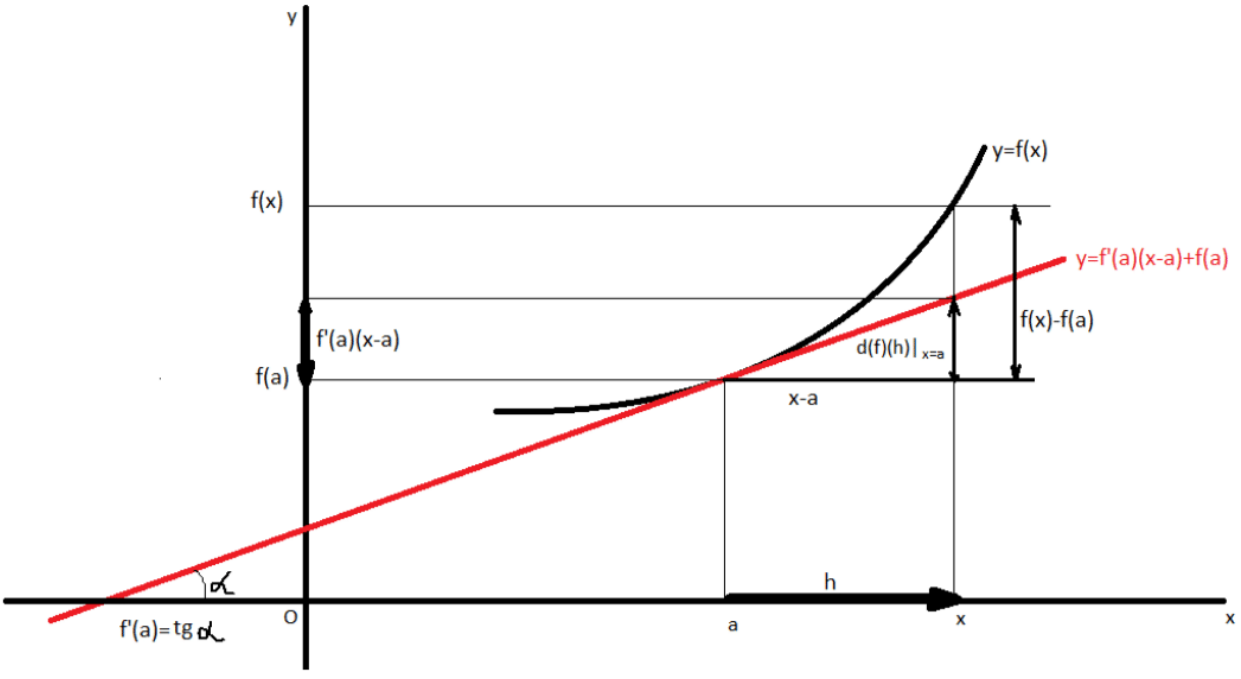
\includegraphics[scale=0.45]{Касательная.png}}
    \caption{Функция "сливается" с касательной.}
    \label{fig:image}
\end{figure} Обратим внимание, что
график функции и касательной неразличимы
в некоторой окрестности.
Приведём несколько примеров на вычисление
производных с помощью определения производной.
\begin{example}
    1) Пусть $f(x)=e^x.$
    Найдём $\frac{df}{dx}(a).$
    Имеем по определению:
    $$
        \frac{df}{dx}(a)=\lim\limits_{h\rightarrow0}
        \frac{e^{a+h}-e^a}{h}=e^a\lim\limits_{h\rightarrow0}
        \frac{e^{h}-1}{h}=e^a.
    $$
    Так как это верно в любой
    точке области определения,
    то при всех $x\in\R$
    $(e^x)'=e^x.$

    2) Пусть $f(x)=\cos x.$ Тогда
    $$
        f'(x)=\lim\limits_{h\rightarrow0}
        \frac{\cos(x+h)-\cos x}{h}=
        \lim\limits_{h\rightarrow0}
        \frac{-2\sin\frac{h}{2}\sin\frac{2x+h}{2}}{h}=
        -\lim\limits_{h\rightarrow0}
        \frac{\sin\frac{h}{2}\sin\frac{2x+h}{2}}
        {\frac{h}{2}}=-\sin x.
    $$
    Совершенно аналогично проверяется, что
    $\sin'(x)=\cos x.$\\
\end{example}

\newpage

\begin{problem}
Доказательство непрерывности дифференцируемой функции. Пример непрерывной и недифференцируемой в точке функции (с доказательством).
\end{problem}

\begin{proposition}
    Пусть функция $f$ дифференцируема
    в точке $a.$ Тогда $f$ непрерывна в точке $a.$
\end{proposition}
\begin{proof}
    Из определения дифференцируемости следует, что
    $$
        f(x)=f(a)+f'(a)(x-a)+o(x-a)\rightarrow f(a), \
        x\rightarrow a,
    $$
    то есть предел функции в точке $a$ равен
    её значению в этой точке, что по определению
    означает непрерывность.
\end{proof}
Следующий пример показывает, что обратное
неверно: непрерывная в точке функция может
быть недифференцируемой в этой точке.
Согласно предложению 1 это равносильно
тому, что такая функция в этой точке не имеет производную.
\begin{example}
    Функция $y=|x|$ недифференцируема в нуле.
    Действительно,
    $$
        \lim\limits_{h\to 0-}
        \frac{|h|}{h}=\lim\limits_{h\to 0-}
        \frac{-h}{h}=-1, \textrm{ а }
        \lim\limits_{h\to 0+}
        \frac{|h|}{h}=
        \lim\limits_{h\to 0-}
        \frac{h}{h}=1.
    $$
    Если бы производная
    в нуле существовала, то есть если бы
    существовал предел, то это было бы равносильно
    существованию и равенству односторонних пределов.
    Таким образом, у функции $y=|x|$
    не существует производной при $x=0,$ что равносильно
    тому, что эта функция недифференцируема в нуле.
\end{example}

\newpage

\begin{problem}
Доказательство правил дифференцирования. Запись этих правил с помощью дифференциалов. Вывод производных функций $f(x) = \tg x, f(x) = \sh x, f(x) = \ch x$.
\end{problem}\begin{proposition}
Пусть функции $f$ и $g$ дифференцируемы
в точке $a.$ Тогда:\\
1) функция $\alpha f+\beta g$ дифференцируема
в точке $a$ при любых $\alpha,\;\beta\in \R$
и $$(\alpha f+\beta g)'(a)=
\alpha f'(a)+\beta g'(a)$$
(свойство линейности);\\
2) $f\cdot g$ дифференцируема в точке $a$
и $(f\cdot g)'(a)=f'(a)g(a)+f(a)g'(a)$
(правило Лейбница);
3) если $g\neq0$ в некоторой окрестности
точки $a,$ то  $\frac{f}{g}$ дифференцируема
в точке $a$ и $\left(\frac{f}{g}\right)'(a)=
\frac{f'(a)g(a)-g'(a)f(a)}{g^2(a)}.$
\end{proposition}
\begin{proof}
1) Найдём производную функции $\alpha f+\beta g$
в точке $a$ по определению, пользуясь арифметикой
пределов:
\begin{multline*}
\lim\limits_{h\rightarrow0}
\frac{(\alpha f+\beta g)(a+h)-
(\alpha f+\beta g)(a)}{h}=\\
=\lim\limits_{h\rightarrow0}
\left(\alpha\frac{f(a+h)-f(a)}{h}
+\beta\frac{g(a+h)-g(a)}{h}\right)=
\alpha f'(a)+\beta g'(a).
\end{multline*}
2) Снова вычислим производную по определению,
используя арифметику пределов:
\begin{multline*}
\lim\limits_{h\rightarrow0}
\frac{f(a+h)g(a+h)-f(a)g(a)}{h}=\\=
\lim\limits_{h\rightarrow0}
\frac{f(a+h)g(a+h)-f(a)g(a+h)+
f(a)g(a+h)-f(a)g(a)}{h}=\\=
\lim\limits_{h\rightarrow0}
\left(g(a+h)\frac{f(a+h)-f(a)}{h}+
f(a)\frac{g(a+h)-g(a)}{h}\right)=\\=
g(a)f'(a)+g'(a)f(a).
\end{multline*}
3) По арифметике пределов имеем:
\begin{multline*}
\lim\limits_{h\rightarrow0}
\frac{f(a+h)/g(a+h)-f(a)/g(a)}{h}=
\lim\limits_{h\rightarrow0}
\frac{f(a+h)g(a)-f(a)g(a+h)}{h}\cdot
\frac{1}{g(a+h)g(a)}=\\=
\frac{1}{(g(a))^2}\cdot\lim\limits_{h\rightarrow0}
\left(g(a)\frac{f(a+h)-f(a)}{h}-
f(a)\frac{g(a+h)-g(a)}{h}\right)=
\frac{f'(a)g(a)-g'(a)f(a)}{g^2(a)}.
\end{multline*}
\end{proof}
Приведём пример применения правил дифференцирования.
\begin{example}
1) Согласно пункту 3)
$$
(\tg x)'=\frac{(\sin x)'
\cos x-(\cos x)'\sin x}{\cos^2x}=
\frac{\cos^2x+\sin^2x}{\cos^2x}=\frac{1}{\cos^2x}
=1+\tg^2x.
$$
Аналогично, $(\ctg x)'=
-\frac{1}{\sin^2x}=-1-\ctg^2x.$\\
2) Рассмотрим полезные функции: гиперболический
синус $\sh x=\frac{e^x-e^{-x}}{2}$ и
гиперболический косинус $\ch x=
\frac{e^x+e^{-x}}{2}.$ Согласно правилам
дифференцирования
$$
(\sh x)'=\frac{1}{2}((e^x)'-(e^{-x})')=
\frac{1}{2}\left(e^x-\left(\frac{1}{e^x}
\right)'\right)=\frac{1}{2}
\left(e^x-\frac{-e^x}{e^{2x}}\right)=
\frac{e^x+e^{-x}}{2}=\ch x.
$$
Аналогично, $(\ch x)'=\sh x.$
\end{example}

\newpage

\begin{problem}
Доказательство теоремы о производной сложной функции. Инвариантность формы
первого дифференциала.
\end{problem}
\begin{proposition}
\textbf{(Производная сложной функции).}
Пусть функция $f$ дифференцируема в точке
$a,$ а функция $g$ дифференцируема в точке
$f(a).$ Тогда функция $g\circ f$ дифференцируема
в точке $a$ и $(g\circ f)'(a)=g'(f(a))\cdot f'(a).$
\end{proposition}
\begin{proof}
Так как функция $g$ дифференцируема в точке
$f(a),$ то при всех $q$ из некоторой
проколотой окрестности нуля
$$
g(f(a)+q)-g(f(a))=g'(f(a))q+\beta(q)q,\;
\lim\limits_{q\rightarrow0}\beta(q)=0.
$$

Доопределим бесконечно малую функцию
$\beta$ в нуле, положив $\beta(0):=0,$
то есть доопределим функцию $\beta$
в нуле по непрерывности.
Теперь мы можем положить
$q=f(a+h)-f(a).$
При этом при подстановке вместо
$q,$ принадлежащего
проколотой окрестности нуля,
приращения $f(a+h)-f(a)$ может возникнуть
ситуация, при которой приращение
для $f$ равно нулю. Для того, чтобы
при этом равенство для приращения $g$
не нарушалось, мы и
доопределили бесконечно малую функцию
$\beta$ в нуле по непрерывности.
Отметим, что такое доопределение не
нарушает дифференцируемость функции $g,$
но позволяет корректно подставить
$q=f(a+h)-f(a).$ 

Тогда
в силу дифференцируемости $f$
(из которой вытекает, что $$f(a+h)-f(a)=
f'(a)h+\alpha(h)h$$ и
$\lim\limits_{h\rightarrow0}\alpha(h)=0$)
в точке $a,$ получим:
\begin{multline*}
g(f(a+h))-g(f(a))=\\
=g'(f(a))(f(a+h)-f(a))+
\beta(f(a+h)-f(a))(f(a+h)-f(a))=\\=
g'(f(a))f'(a)h+g'(f(a))\alpha(h)h+
\beta(f'(a)h+\alpha(h)h)(f'(a)h+\alpha(h)h)=\\
=g'(f(a))f'(a)h+\delta(h)h.
\end{multline*}
Мы использовали обозначение
$\delta(h)=g'(f(a))\alpha(h)+
\beta(f'(a)h+\alpha(h)h)(f'(a)+\alpha(h)),$
а тогда из арифметики пределов и из
бесконечной малости функций $\beta$
и $\alpha$ следует, что $\delta(h)
\rightarrow0,\;h\rightarrow0.$
Таким образом, для функции $g\circ f$
получим при достаточно малых $h:$
$$
g(f(a+h))-g(f(a))=
g'(f(a))f'(a)h+\delta(h)h,
$$
что даёт дифференцируемость
функции $g\circ f$ в точке $a$ по определению.
Мы знаем, что это равносильно
наличию у функции $g\circ f$ производной
в точке $a.$ Таким образом, получаем,
что $(g\circ f)'(a)=
g'(f(a))f'(a).$
\end{proof}
В некоторой точке $y,$ в которой
дифференцируема функция $g,$
мы можем записать дифференциал
функции $g$ в виде $dg(y)=g'(y)dy$
(см. предыдущую лекцию). Пусть
$f$ дифференцируема в точке $x$
и $f(x)=y.$ Теорема
о производной сложной функции тогда
в терминах дифференциалов запишется
так (в точке $x$):
$$
d(g\circ f)(x)=g'(f(x))f'(x)dx=
g'(f(x))df(x)=g'(y)dy.
$$
Таким образом, вне зависимости от того, является
ли $y$ независимой переменной или функцией,
форма (то есть вид) первого дифференциала
внешне не меняется. Это свойств
дифференциала называется
\textbf{\emph{инвариантностью формы первого
дифференциала.}}
\newpage

\begin{problem}
Доказательство теоремы о производной обратной функции. Выводы формул таблицы
производных.
\end{problem}
\begin{proposition}
\textbf{(Производная обратной функции).}
Пусть $f$ -- непрерывная и строго монотонная функция,
отображающая интервал $I$ в интервал $J.$ Пусть также
$f$ дифференцируема в точке $a\in I$ и $f'(a)\neq0.$
Тогда обратная функция $f^{-1}$ дифференцируема
в точке $b=f(a)$ и $(f^{-1})'(b)=\frac{1}{f'(a)}.$
\end{proposition}
\begin{proof}
Существование, непрерывность и монотонность
функции $f^{-1}$ следует из теоремы об
обратной функции.
Воспользуемся определением производной, считая, что
аргумент функции $f^{-1}$ получает приращение $q,$
а затем положим $q=f(a+h)-f(a)$ и воспользуемся
теоремой о пределе композиции и арифметикой
пределов:
\begin{multline*}
\lim\limits_{q\rightarrow0}
\frac{f^{-1}(f(a)+q)-f^{-1}(f(a))}{q}=
\lim\limits_{h\rightarrow0}
\frac{f^{-1}(f(a)+(f(a+h)-f(a)))-f^{-1}(f(a))}
{f(a+h)-f(a)}=\\=
\lim\limits_{h\rightarrow0}
\frac{a+h-a}
{f(a+h)-f(a)}=\frac{1}{f'(a)}.
\end{multline*}
При этом $f(a+h)-f(a)\neq0$
при $h\neq0,$ так как функция
$f$ строго монотонна.
\end{proof}
В дифференциалах формула запишется так:
$df^{-1}(f(a))=(df(a))^{-1}$
(что следует из формулы
$df^{-1}(f(a))(h)=\frac{1}{f'(a)}h,$
тогда как $df(a)(h)=f'(a)h,$
то есть линейные функции
$df(a)$ и $df^{-1}(f(a))$
взаимно обратны).
\begin{example}
1) Пусть $\tg y=x$, тогда
при $x\in\left(-\frac{\pi}{2},
\frac{\pi}{2}\right)$ $y=\arctg x.$
По теореме о производной обратной
функции $(\arctg x)'=\frac{1}
{(\tg y)'}=\frac{1}{1+(\tg y)2}=
\frac{1}{1+x^2}.$
Аналогично проверяется, что
$(\arcsin x)'=-(\arccos x)'=
\frac{1}{\sqrt{1-x^2}}.$\\
2) Пусть $e^y=x$, тогда
$\ln x=y.$ $(\ln x)'=
\frac{1}{(e^y)'}=
\frac{1}{x}.$\\
3) Теперь, зная производную логарифма,
при любом вещественном $\alpha$ из
теоремы о производной сложной функции
имеем $(x^{\alpha})'=
(e^{\alpha\ln x})'=
e^{\alpha\ln x}\cdot\alpha
\cdot\frac{1}{x}=\alpha x^{\alpha-1}.$
\end{example}
Теперь выпишем \textbf{таблицу производных,}
все равенства в которой либо уже выведены
с использованием наших теорем, либо
выводятся аналогично. При этом в основании
логарифма и показательной функции мы считаем,
что $a>0, \ a\neq1,$ а все функции рассматриваются
на своих областях определения.
\begin{multline*}
{\bf 1)} \ C'=0\;\forall C=const; \ {\bf 2)} \ (x^{\alpha})'=
\alpha x^{\alpha-1}; \ {\bf 3)} \ (e^x)'=e^x; \ {\bf 4)} \ (a^x)'=
a^x\ln a; \ {\bf 5)} \ (\ln x)'=1/x;\\
{\bf 6)} \ (\log_a x)'=
\frac{1}{x\ln a}; \ {\bf 7)} \ (\sin x)'=\cos x; \
{\bf 8)} \ (\cos x)'=-\sin x; \ {\bf 9)} \ (\tg x)'=
\frac{1}{\cos^2x}=\tg^2x+1;\\
{\bf 10)} \ (\ctg x)'=-\frac{1}{\sin^2x}=-\ctg^2x-1; \
{\bf 11)} \ (\arcsin x)'=\frac{1}{\sqrt{1-x^2}}; \
{\bf 12)} \ (\arccos x)'=-\frac{1}{\sqrt{1-x^2}};\\
{\bf 13)} \ (\arctg x)'=\frac{1}{1+x^2}; \
{\bf 14)} \ (\arcctg x)'=-\frac{1}{1+x^2}; \
{\bf 15)} \ (\sh x)'=\ch x; \
{\bf 16)} \ (\ch x)'=\sh x.
\end{multline*}
\newpage

\begin{problem}
Доказательства теорем Ферма и Ролля. Примеры к невыполнению условий теоремы
Ролля.
\end{problem}
Теорема 1. (Теорема Ферма). Пусть функция $f$ определена на интервале $(a, b)$, дифференцируема в точке $c \in(a, b)$ и имеет в точке с локальный экстремум. Тогда $f^{\prime}(c)=0$.

Доказательство. Пусть в точке $c$ функция $f$ имеет максимум (для минимума доказательство аналогично). Тогда при всех $x>c$ справедливо неравенство $\frac{f(x)-f(c)}{x-c} \leq 0$, а при всех $x<c-$ неравенство $\frac{f(x)-f(c)}{x-c} \geq 0$. Так как существует производная функции $f$ в точке $c$, то есть существует предел $\lim _{x \rightarrow c} \frac{f(x)-f(c)}{x-c}=f^{\prime}(c)$, то существуют и равны друг другу оба односторонних предела: $\lim _{x \rightarrow c-} \frac{f(x)-f(c)}{x-c}=f^{\prime}(c)=\lim _{x \rightarrow c+} \frac{f(x)-f(c)}{x-c}$. Таким образом, из предельного перехода в неравенствах имеем
$$
\left(f^{\prime}(c)\right)^2=\lim _{x \rightarrow c-} \frac{f(x)-f(c)}{x-c} \cdot \lim _{x \rightarrow c+} \frac{f(x)-f(c)}{x-c} \leq 0,
$$

что равносильно тому, что $f^{\prime}(c)=0$.
Теорема 2. (Теорема Ролля). Пусть:
1) Функция $f$ определена и непрерывна на отрезке $[a, b]$.
2) Функция $f$ дифферениируема на интервале $(a, b)$.
3) $f(a)=f(b)$.

Тогда существует такая точка $c \in(a, b)$, что $f^{\prime}(c)=0$.

Доказательство. Если функция непрерывна на отрезке $[a, b]$, то по второй теореме Вейерштрасса существуют такие точки $c_1 \in[a, b]$ и $c_2 \in[a, b]$, что $f\left(c_1\right)=m:=\inf _{a \leq x \leq b} f(x)$ и $f\left(c_2\right)=M:=\sup _{a \leq x \leq b} f(x)$. Если при этом $m=M=f(a)$, то функция $f$ на отрезке $[a, b]$ является постоянной, поэтому в любой точке интервала $(a, b)$ её производная равна нулю. Если $m<M$, то хотя бы одна из точек $c_1$ и $c_2$ лежит в интервале $(a, b)$ и согласно теореме Ферма производная функции $f$ в этой точке равна нулю. Эту точку и можно взять в качестве $c$.
Все условия теоремы Ролля важны. Если отказаться от условия 1) (при выполнении условий 2) и 3)), то можно рассмотреть функцию $f$, удовлетворяющую равенству
$$
f(x)=\left\{\begin{array}{l}
x, \text { если } x \in[0,1), \\
0, \text { если } x=1 .
\end{array}\right.
$$
(см. рисунок 1). Производная этой функции равна 1 в каждой точке интервала $(0,1)$.
Рис. 1: Функция разрывна на отрезке, но дифференцируема на интервале
Если взять непрерывную на отрезке $[-1,1]$ функцию, но отказаться от дифференцируемости на интервале, то подойдёт функция $y=|x|$, но утверждение теоремы Ролля для неё не выполнено. Наконец, если отказаться от условия 3), то можно на любом отрезке просто взять функцию $y=x$, производная которой ни в одной точке не обращается в нуль.
\newpage

\begin{problem}
Доказательства теоремы Лагранжа и её следствий.
\end{problem}
Теорема 3. (Теорема Лагранжа). Пусть:
1) Функиия $f$ определена и непрерывна на отрезке $[a, b]$.
2) Функция $f$ дифференцируема на интервале $(a, b)$.

Тогда существует такая точка $c \in(a, b)$, что $f(b)-f(a)=f^{\prime}(c)(b-a)$.
Доказательство. Рассмотрим функцию $g$, определяемую равенством
$$
g(x)=f(x)-f(a)-\frac{f(b)-f(a)}{b-a}(x-a) .
$$

Эта функция по свойствам непрерывных и дифференцируемых функций непрерывна на отрезке $[a, b]$, дифференцируема на интервале $(a, b)$ и $g(a)=0=g(b)$. Таким образом, функция $g$ удовлетворяет всем условиям теоремы Ролля на $[a, b]$, поэтому существует такая точка $c \in(a, b)$, что $g^{\prime}(c)=0$, а это равносильно тому, что $f^{\prime}(c)=\frac{f(b)-f(a)}{b-a}$.

Предложение 1. (1-е следствие) Пусть функция $f$ определена и дифференцируема на интервале $(a, b)$ и $f^{\prime}(x)=0 \forall x \in(a, b)$. Тогда функция $f$ постоянна на $(a, b)$.

Доказательство. Пусть $x_1, x_2 \in(a, b), x_1<x_2$. Тогда на отрезке $\left[x_1, x_2\right]$ к функции $f$ применима теорема Лагранжа, поэтому $f\left(x_2\right)-f\left(x_1\right)=f^{\prime}(c)\left(x_2-x_1\right)$, где $c \in\left(x_1, x_2\right)$. По условию $f^{\prime}(c)=0$, поэтому $f\left(x_1\right)=f\left(x_2\right)$. Так как рассуждение верно для любых точек на интервале $(a, b)$, то, зафиксировав $x_1$ и беря произвольные значения $x_2 \in(a, b)$, видим, что во всех точках интервала функция $f$ принимает равные значения.
Предложение 2. (2-е следствие) Пусть функция $f$ определена и дифференцируема на интервале $(a, b)$.
1) Функция $f$ не убывает на этом интервале тогда и только тогда, когда
$$
f^{\prime}(x) \geq 0 \forall x \in(a, b) .
$$
2) Функция $f$ не возрастает на этом интервале тогда и только тогда, когда
$$
f^{\prime}(x) \leq 0 \forall x \in(a, b) .
$$

Доказательство. Проведём доказательство для случая неубывающей функции (для невозрастающей всё аналогично).

Необходимость. Если функция не убывает на интервале $(a, b)$, то для любых точек
$$
x_1, x_2 \in(a, b),
$$

имеем:
$$
\frac{f\left(x_2\right)-f\left(x_1\right)}{x_2-x_1} \geq 0 .
$$

Зафиксировав точку $x_1$, получим в силу предельного перехода в неравенствах, что
$$
\lim _{x_2 \rightarrow x_1} \frac{f\left(x_2\right)-f\left(x_1\right)}{x_2-x_1}=f^{\prime}\left(x_1\right) \geq 0 .
$$

В силу произвольности точек $x_1$ и $x_2$ получаем неотрицательность $f^{\prime}$ в каждой точке интервала $(a, b)$.
Достаточность. Если $f^{\prime}(x) \geq 0 \forall x \in(a, b)$, то по теореме Лагранжа
$$
f\left(x_2\right)-f\left(x_1\right)=f^{\prime}(c)\left(x_2-x_1\right) \geq 0
$$

при всех $x_1, x_2 \in(a, b), x_1<x_2$.
\newpage

\begin{problem}
Доказательство теоремы Коши и её физический смысл.
\end{problem}
Теорема 4. (Теорема Коши). Пусть функции $f$ и g:
1) определены и непреръвны на отрезке $[a, b]$;
2) дифференцируемы на интервале $(a, b)$;
3) $g^{\prime}(x) \neq 0 \forall x \in(a, b)$.

Тогда сущестөует точка такая точка $c \in(a, b)$, что $\frac{f(b)-f(a)}{g(b)-g(a)}=\frac{f^{\prime}(c)}{g^{\prime}(c)}$.
Доказательство. Отметим прежде всего, что $g(a) \neq g(b)$, так как в противном случае функция $g$ удовлетворяет всем условиям теоремы Ролля, поэтому условие 3) теоремы выполняться не может.

Снова сведём доказательство к теореме Ролля. Рассмотрим вспомогательную функцию $G$, определяемую равенством
$$
G(x)=(g(b)-g(a)) f(x)-(f(b)-f(a)) g(x) .
$$

Эта функция непрерывна на отрезке $[a, b]$, дифференцируема на интервале $(a, b)$ и
$$
G(a)=g(b) f(a)-g(a) f(b)=G(b),
$$

то есть все условия теоремы Ролля выполнены. Тогда найдётся такая точка $c \in(a, b)$, что
$$
G^{\prime}(c)=(g(b)-g(a)) f^{\prime}(c)-(f(b)-f(a)) g^{\prime}(c)=0,
$$

откуда и получается доказываемое равенство.

Отметим, что если убрать условие 3) теоремы Коши, то можно доказать, что будет справедливо равенство $f^{\prime}(c)(g(b)-g(a))=g^{\prime}(c)(f(b)-f(a))$. Это равенство равносильно тому, что
$$
\left|\begin{array}{ll}
f(b)-f(a) & f^{\prime}(c) \\
g(b)-g(a) & g^{\prime}(c)
\end{array}\right|=0 .
$$

Равенство нулю определителя означает, что столбцы матрицы образуют коллинеарные векторы, а отсюда можно получить один из возможных физических смыслов задачи Ко$u u$ : если вектор $(f(x), g(x))$ - это закон движения тела на плоскости, а $x$ играет роль времени, то вектор $(f(b)-f(a), g(b)-g(a))$ будет вектором перемещения за время $b-a$, а вектор $\left(f^{\prime}(c), g^{\prime}(c)\right)$ - это вектор мгновенной скорости в момент времени $c$. Таким образом, в теореме Коши утверждается, что вектор перемещения коллинеарен вектору мгновенной скорости, взятому в какой-то момент времени между моментами $a$ и $c$. В трехмерном пространстве в общем случае это не верно (например, при движении по винтовой линии на поверхности цилиндра).
\newpage
